\documentclass[a4paper, 11pt, fleqn, normalem]{report}

\usepackage{../../LaTeX-Templates/Notes}

\setcounter{tocdepth}{1}
\setcounter{secnumdepth}{1}

\title{Foundations of Physics Year 1 \\ Waves and Optics \vspace{-20pt}}
\author{Ruth Gregory}
\date{\vspace{-15pt}Michaelmas Term 2016}

\begin{document}

\maketitle
\thispagestyle{fancy}

\tableofcontents

\newpage
\section{Mechanical Waves}
Mechanical Waves propagate through/on a system \\
Typically, the medium oscillates in a particular fashion:
\begin{itemize}
    \item Transverse waves: Oscillations are perpendicular to the direction of motion
    \item Longitudinal waves: Oscillations are parallel to the direction of motion
\end{itemize}

\section{Harmonic Waves}
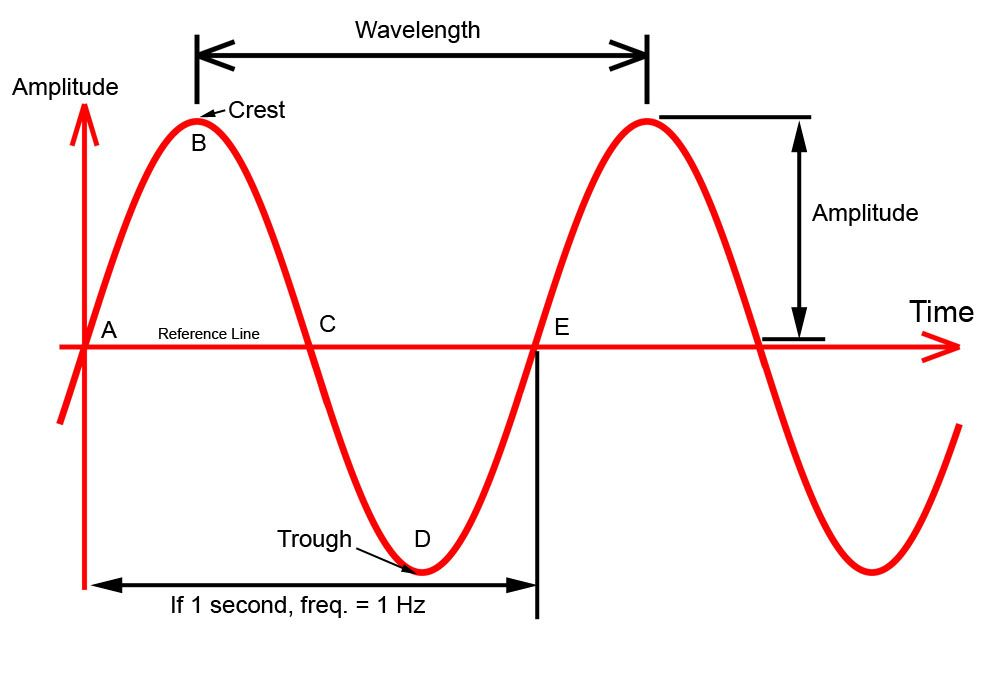
\includegraphics[scale=0.3]{Sine.jpg} \\
Point A shows the driver that generates the wave: each wave undergoes Simple Harmonic Motion \\
Wavelength -- $\lambda$; Frequency -- f; Angular frequency -- $\omega = 2{\pi}f$; \\
Amplitude -- A; Period -- $T = 1 \frac{\lambda}{s} = \frac{1}{f} = \frac{2\pi}{\omega}$; Velocity -- $v = \frac{\lambda}{T} = {\lambda}f$

Basic mathematical form of a wave is $y = f(x \mp vt)$ -- minus for moving right, plus for moving left \\
Can model any wave as $y = f(x,\,t)$

For a SHM driver:
\begin{equation*}
    {\delta}y = A\cos{({\omega}t + \phi)}
\end{equation*}
This tells us for the wire that $y(0,\,t) = A\cos{({\omega}t)} ~\because~ \phi = 0$ \\
The wave travels to the right, so y is a function of $(x-vt)$:
\begin{gather*}
    y = f(x-vt) \\
    y(0,\,t) = f(-vt) = A\cos{{\omega}t} \\
    \implies y(x,\,t) = A\cos{\Big(\frac{\omega}{v}(x-vt)\Big)} = A\cos{\Big(\frac{\omega}{v}x - {\omega}t\Big)} \\
    \implies y(x,\,t) = A\cos{\Big(2\pi\Big(\frac{x}{\lambda} - ft\Big)\Big)}
\end{gather*}
This shows periodicity in x \& t \\
Define the \underline{wave number}, $k = \frac{2\pi}{\lambda}$ -- this is the analogue of $\omega$ for x
\begin{equation*}
    \implies y(x,\,t) = A\cos{(kx - {\omega}t)} \text{ [For a harmonic wave moving to the right]}
\end{equation*}

\section{The Wave Equation}
Guess work from the previous equation gives:
\begin{align*}
    \dot{y}(x,\,t) &= \pm A{\omega}\sin{(kx \mp {\omega}t)}                 & y'(x,\,t) &= \pm Ak\sin{(kx \mp {\omega}t)} \\
    \ddot{y}(x,\,t) &= -A\omega^{2}\cos{(kx \mp {\omega}t)} = -A\omega^{2}y & y''(x,\,t) &= -Ak^{2}\sin{(kx \mp {\omega}t)} = -Ak^{2}y
\end{align*}
Since $\frac{\delta y}{\delta(x,\,t)}$ changes sign for left- \& right-moving waves, cannot use the wave equation
\begin{equation*}
    \text{But } \ddot{y} - \frac{\omega^{2}}{k^{2}}y'' = 0 ~~[\frac{\omega^{2}}{k^{2}} = v^{2}]
\end{equation*}
From this, the maths for a wire under a tension, F, can be derived:\\
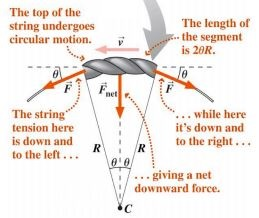
\includegraphics{Tension.jpg} \\
Resolve forces on the left- and right-hand sides:
\begin{align*}
         R&HS                  &      L&HS                   \\
    x_{0} &+ {\delta}x         &      x&_{0}                 \\
    F_{x} &= F\cos{\theta_{2}} & F_{x} &= -F\cos{\theta_{1}} \\
    F_{y} &= F\sin{\theta_{2}} & F_{y} &= -F\sin{\theta_{1}}
\end{align*}
Use the small angle approximation: $\cos{\theta} \approx 1$, $\sin{\theta} \approx \theta$
\begin{gather*}
    \therefore F_{Tot\,x} = F(\cos{\theta_{2}} - \cos{\theta_{1}}) \approx 0 \\
    F_{Tot\,y} = F(\sin{\theta_{2}} - \sin{\theta_{1}}) \approx F(\theta_{2} - \theta_{1}) \\
    ~~~~~~~\,\approx F(\tan{\theta_{2}} - \tan{\theta_{1}})
\end{gather*}
But $\tan{\theta}$ is the gradient of the wire at each end:
\begin{gather*}
    F_{Tot\,y} = F\Big(\frac{{\delta}y}{{\delta}x}\Big|_{x_{0} + {\delta}x} - \frac{{\delta}y}{{\delta}x}\Big|_{x_{0}}\Big)
\end{gather*}
But recall when differentiating:
\begin{equation*}
    \frac{df}{dx} = \lim_{h\to0} \frac{f(x+h) - f(h)}{h}
\end{equation*}
Here, $h = {\delta}x$ and $f = \frac{{\delta}y}{{\delta}x}$
\begin{gather*}
    \implies \frac{{\delta}y}{{\delta}x}\Big|_{x_{0} + {\delta}x} - \frac{{\delta}y}{{\delta}x}\Big|_{x_{0}} \approx~ \delta x \frac{\delta^{2}y}{\delta x^{2}} \\
    \implies F_{Tot\,y} = F\delta x\frac{\delta^{2}y}{\delta x^{2}}
\end{gather*}
Meanwhile, $F_{Tot\,y} = ma \rightarrow \mu\delta x \frac{\delta^{2}y}{\delta t^{2}}$, where $\mu$ is the mass per unit length
\begin{gather*}
    \implies F\frac{\delta^{2}y}{\delta x^{2}} \delta x = \mu\delta x\frac{\delta^{2}y}{\delta t^{2}}
\end{gather*}
The wave equation, therefore, is
\begin{gather*}
    \underline{\frac{\delta^{2}y}{\delta t^{2}} = \frac{F}{\mu}\frac{\delta^{2}y}{\delta x^{2}}}
\end{gather*}
where:
\begin{gather*}
    v^{2} = \frac{F}{\mu}
\end{gather*}

\section{Energy In Wave Motion}
As a wave moves, it transmits energy \\
At constant amplitude, energy is transmitted at a constant rate \\
Calculating for a harmonic wave: $y(x,\,t) = A\cos{(kx - \omega t)}$ \& $E_{tot} = KE + PE$ \\
Look at little piece of wire, $\delta x \rightarrow$ vibrates up, then falls back down
\begin{equation*}
    \delta E_{KE} = \frac{1}{2}\delta mv^{2} = \frac{1}{2}\mu\delta x\dot{y}^{2}
\end{equation*}
Evaluate total energy when $PE = 0$, i.e. the wire is at the equilibrium position $\implies$ \\
$\dot{y}$ is maximised so when $y = 0$, $\cos{(kx - \omega t)} = 0 ~\therefore~ kx - \omega t = \frac{\pi}{2} + n\pi ~\forall~ n \in \mathbb{R}$
\begin{gather*}
    \implies \dot{y}(x,\,t) = A\omega\sin{(kx - \omega t)} \\
    \implies \dot{y} = \pm A\omega \\
    \implies \delta E_{KE} = \frac{1}{2}\mu\delta xA^{2}\omega^{2}
\end{gather*}
Wave moves to the right at a constant velocity, so $\Delta x = v \,\Delta t$ gives distance through which energy propagates in time $\Delta t$ \\
So energy is given by: $\underline{\delta E = \frac{1}{2}\mu vA^{2}\omega^{2}\,\delta t}$ \\
The rate at which energy is transmitted, or the transmission power P, is:
\begin{gather*}
    P = \frac{dE}{dt} = \frac{1}{2}\mu A^{2}\omega^{2}v \\
    \therefore ~\underline{P = \frac{1}{2}\sqrt{\mu F}A^{2}\omega^{2}}
\end{gather*}

\section{Wave Intensity}
For waves propagating through the unconfined media, intensity is a more useful concept than power \\
Intensity is defined as the rate of energy transmission per unit area, $I = \frac{P}{A}$ \\
For a spherical wavefront, $I = \frac{P}{4\pi r^{2}}$ \\
The total energy output rate is constant but spread over a larger area \\
This underlies the "standard candle" principal for distance in cosmology \\
Inverse square law for intensity:
\begin{equation*}
    4\pi r^{2}_{1}I_{1} = 4\pi r^{2}_{2}I_{2}
\end{equation*}

\section{Waves At Boundaries}
Waves reflect at boundaries \\
How they reflect depends on the nature of the boundary \\
Fixed boundaries return opposite amplitude wave -- $y(x,\,t) = A\cos{(kx - \omega t)} + B\cos{(kx + \omega t)}$ \\
Fixed at a boundary means $y(0,\,t) = 0 = A\cos{(\omega t)} + B\cos{(-\omega t)} \implies A = -B$ \\
Therefore left-moving is inverted relative to right-moving wave

Free boundaries returns same amplitude -- consider a string attached to a pole by an unfixed ring.
The ring moves up and down with the wave. \\
Wire is always horizontal at transition: $\frac{\delta y(0,\,t)}{\delta x} = y'(0,\,t) = 0$
\begin{gather*}
    y'(0,\,t) = [-Ak\sin{(kx - \omega t)} - Bk\sin{(kx + \omega t)}]_{x = 0} \\
    y'(0,\,t) = Ak\sin{(\omega t)} - Bk\sin{(\omega t)} = 0 \\
    \therefore~ A - B = 0 \implies A = B
\end{gather*}

\section{Superposition of Waves}
The wace equation is linear so:
\begin{gather*}
    \frac{\delta^{2}}{\delta t^{2}}(y_{1} + y_{2}) = \ddot{y}_{1} + \ddot{y}_{2} \\
    = v^{2}y''_{1} + v^{2}y''_{2} = v^{2}\frac{\delta^{2}}{\delta x^{2}}(y_{1} + y_{2})
\end{gather*}
If $y_{1}$ and $y_{2}$ both satisfy the wave equation, then so does $y_{1} + y_{2}$ \\
This implies the \emph{principal of Superposition}

\section{Standing Waves On A String}
Standing waves occurs when left- \& right-moving waves with the same frequency \& amplitude interfere
\begin{gather*}
    y = A[\sin{(kx - \omega t)} + \sin{(kx + \omega t)}] = 2A\sin{(kx)}\cos{(\omega t)} \\
    y(0,\,t) = 0;\;\,y\Big(\frac{n\pi}{k},\,t\Big) = 0
\end{gather*}
For length $\frac{n\pi}{k}$ of wire, $y(L,\,t) = 0$ \\
y is also zero when $kx = n\pi,~\{ n \in \mathbb{N}\}$ -- these points are called nodes \\
Maximal displacement is at an anti-node -- $kx = \Big(n + \frac{1}{2}\Big)\pi$ \\
Waves reflecting off fixed ends of string generate normal modes -- they start \& finish at boundaries of L \\
End points are nodes, so $L = \frac{n\lambda\pi}{2}$
\begin{gather*}
    f_{n} = \frac{v}{\lambda n} = \frac{nv}{2L} \\
    f_{1} = \frac{1}{2L}\sqrt{\frac{F}{\mu}}\text{ -- fundamental frequency}
\end{gather*}

\section{Sound \& Hearing}
Sound is a sinusoidal longitudinal wave, usually travelling through air: $y(x,\,t) = A\cos{(kx - \omega t)}$
Use this to find the pressure wave and velocity:
\begin{gather*}
    y'(x,\,t) = -Ak\sin{(kx - \omega t)} \\
    \dot{y}(x,\,t) = A\omega\sin{(kx - \omega t)} \\
    \dot{y} = -\frac{\omega}{k}y' = -vy'
\end{gather*}
$\Delta$P is given by $\Delta$V and the bulk modulus:
\begin{gather*}
    \delta P = -B\frac{\delta V}{V} \\
    V = S\delta x \text{ where S is the area through which the sound wave moves}\\
    \delta V = S(y(x_{0} + \Delta x,\, t) - y(x_{0},\, t)) = S\Delta x \frac{\delta y}{\delta x}\Big|_{x_{0}} \\
    \delta P = -B\frac{\delta y}{\delta x} = Bk\sin{(kx - \omega t)} \\
    \therefore~ P_{max} = BkA
\end{gather*}
For speed, relate $\delta$P to velocity differential:
\begin{gather*}
    \delta P = \frac{\delta F}{A} = \frac{1}{S}\frac{\delta p}{\delta t} \\
    \delta p = \delta m\dot{y} \\
    \delta p = \rho\times S\Delta x\times\dot{y} \\
    -By' = \frac{\rho\Delta x\dot{y}}{\delta t} = -v^{2}\rho y' \\
    v^{2} = \frac{B}{\rho} \\
    v = \sqrt{\frac{B}{\rho}}
\end{gather*}
Recall that for ideal gases, $pV = nRT$ and the isothermal bulk modulus, $B = p \implies$
\begin{gather*}
    v^{2} = \frac{nRT}{M} \\
    v = \sqrt{\frac{nRT}{M}}
\end{gather*}
In a solid, use Young's Modulus:
\begin{equation*}
    v = \sqrt{\frac{Y}{\rho}}
\end{equation*}

\section{Sound Intensity}
Rate at which waves transport energy per unit area per unit time
\begin{gather*}
    \delta E = F\:\delta x = \delta P\times \delta S\times \delta x \\
    \text{Intensity, } I = \frac{\delta E}{\delta S\,\delta t} = \frac{\delta P\,\delta S\,\delta x}{\delta S\,\delta t} \\
    \implies I = -By'\dot{y} BkA\sin{(kx - \omega t)}\times\omega A\sin{(kx - \omega t)} \\
    \implies I = Bk\omega A^{2}\sin^{2}{(kx - \omega t)}
\end{gather*}
Looking for $\langle I\rangle$:
\begin{gather*}
    \langle\sin^{2}\rangle = \frac{1}{2} \\
    I = \frac{1}{2}Bk\omega A^{2} \\
    k = \frac{\omega}{v} = \omega\sqrt{\frac{\rho}{B}} \\
    I = \frac{1}{2}\sqrt{\rho B}\omega^{2}A^{2}
\end{gather*}

\section{The Decibel Scale}
Humans can detect sounds in a range of around 12 orders of magnitude so it easier to use a logarithmic scale:
\begin{equation*}
    \beta = 10\log{\frac{I}{I_{0}}}
\end{equation*}
$I_{0} = 10^{-12} W\:m^{-2} ~\therefore~ 0 \rightarrow 120dB$ is hearing range

\section{Standing Waves and Normal Nodes}
Sound Waves in pipes reflect from ends and interfere to form standing waves \\
Nodes \& anti-nodes --
Node: no air motion/maximum pressure variation; anti-node: maximal air motion/no pressure variation \\
There is a node at the end of a closed pipe and an anti-node at the end of an open pipe \\
2 open ends: anti-node at either end with a node in the middle; $\lambda = 2L$ \\
1 open end, 1 closed end: node at closed end, anti-node at open end; $\lambda = 4L$ \\
Odd harmonics in 1 open, 1 closed (harmonics giving using fundamental frequency equation)

\section{Sound Phenomena}
Sound waves interfere via principe of superposition \\
Phase and frequency are both important \\
For 2 waves of same amplitude and frequency, they can be: \\
'in-phase' for constructive interference; 'out-of-phase' for destructive interference
\begin{gather*}
    y_{1} = A\cos{(kx - \omega t)} \\
    y_{2} = A\cos{(kx - \omega t + \phi)}
    y_{1} + y_{2} = A\Big[\cos{\Big(kx - \omega t + \frac{\phi}{2} - \frac{\phi}{2}\Big)} + \cos{\Big(kx - \omega t + \frac{\phi}{2} + \frac{\phi}{2}\Big)}\Big] \\
    y_{1} + y_{2} = 2A\Big[\cos{\Big(kx - \omega t + \frac{\phi}{2}\Big)}\cos{\Big(\frac{\phi}{2}\Big)}\Big]\text{ -- Oscillatory with amplitude }2A\cos{\Big(\frac{\phi}{2}\Big)}
\end{gather*}
The most common reason for phase difference is path length

\section{Beats}
When 2 waves are very nearly equal frequencies, beats occur
Sitting at $x = 0$:
\begin{gather*}
    y_{1} = A\cos{(2\pi f_{1}t)} \\
    y_{2} = A\cos{(2\pi f_{2}t)} \\
    f_{2} = f_{1} + \delta f
\end{gather*}
Think of effect of $\delta f$ as producing time-depended phase, $\phi \approx \delta ft$
\begin{gather*}
    y_{1} + y_{2} = A[\cos{(2\pi(f_{1} + \delta f)t)} + \cos{(2\pi f_{1}t)}] \\
    = 2A\cos{(\pi\delta ft)}\cos{\Big(2\pi\Big(f_{1} + \frac{\delta f}{2}\Big)t\Big)}
\end{gather*}
This is nearly the same pitch as the orginal, the amplitude varies slowly over time \\
Consider the period of cos:
\begin{gather*}
    T = \frac{2\pi}{\pi\delta f} = \frac{2}{\delta f} \\
    \therefore T >> \frac{1}{f_{1}} \\
    f_{beat} = f_{2} - f_{1} = \delta f
\end{gather*}
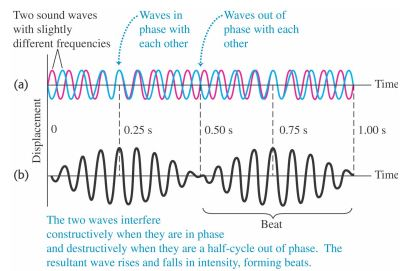
\includegraphics[scale=0.8]{Beat.jpg}

\section{The Doppler Effect}
A shift in pitch due to motion \\
Key observation is that sound is transmitted through a medium that has a rest frame \\
Shift occurs whether it is listener source that is moving, though the effect is different in each case

For a moving source: \\
$f_{s}$ is fixed \\
Intuition -- waves bunch up in front of the source and spread out behind
\begin{align*}
    \text{For}&\text{ward: } & \lambda_{f} =& \frac{c_{f}}{f_{s}} = \frac{c - v_{s}}{f_{s}} & f_{L} = \frac{c}{\lambda_{L}} =& \frac{c}{\lambda_{f}} = \frac{c}{c - v_{s}}f_{s} > f_{s} \\
    \text{Ba}&\text{ck: } & \lambda_{b} =& \frac{c + v_{s}}{f_{s}} & f_{b} = \frac{c}{\lambda_{b}} =& \frac{c}{c + v_{s}}f_{s} > f_{s}
\end{align*}
For a moving listener: \\
$\lambda_{s}$ is fixed \\
Intuition -- listener is either catching up or receding from the wave, increasing/decreasing sound speed
\begin{gather*}
    \text{Forward: } f_{L} = \frac{c_{L}}{\lambda_{s}} = \frac{c + v_{L}}{c}f_{s} \\
    \text{Back: } f_{L} = \frac{c - v_{L}}{c}f_{s}
\end{gather*}
In general:
\begin{equation*}
    f_{L} = \frac{c \pm v_{L}}{c \pm v_{s}}f_{s}
\end{equation*}
If medium moves, $c \rightarrow c \pm v_{medium}$

Examples: \\
Doppler flow meter -- high frequency sound emitted towards body, reflected back to reciever allowing for exomaple inmaging of blood flow

\section{The Nature and Propagation of Light}
Light is an electromagnetic wave -- oscillations between electric and magnetic components \\
Light as a wave: satisfies the wave equation, has interference and diffraction; \\
Light as a particle: multiple of finite energy, E = hf \\
Wave Equation: $\frac{\delta^{2}}{\delta t^{2}}\underline{E} = c^{2}\underline{\nabla}^{2}\underline{E};~\&~ \frac{\delta^{2}}{\delta t^{2}}B = c^{2}\underline{\nabla}^{2}\underline{B}$ \\
This can be derived from a guage potential: $\underline{E} = \underline{\nabla}\phi + \frac{d\underline{A}}{dt};~\&~\underline{B} = \underline{\nabla}\times\underline{A}$ \\
Visible light is a small part of the electromagnetic spectrum, with all wavelengths travelling at the same speed through a vacuum -- $c \approx 3\times10^{8}\:m\:s^{-1}$ \\
Light slows down in a different medium -- $c = \frac{1}{\sqrt{\epsilon\mu}}$\\
c is not frame-dependent, c is fundamental

\section{Reflection and Refraction}
Light slows down in a medium, encoded in the refractive index
\begin{equation*}
    n = \frac{c}{v_{m}} \geq 1
\end{equation*}
When light hits interface between two media, some reflects, some doesn't \\
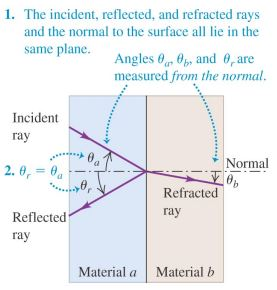
\includegraphics{Incidence.jpg} \\
Incident, refracted, and reflected rays are all in same plane \\
$\theta_{r} = \theta_{i}$ for reflection \\
For refraction, Snell's Law describes the relationship \\
This is easily derived from Fermat's principal of Least Action: Light takes "least-time path" between two points\\
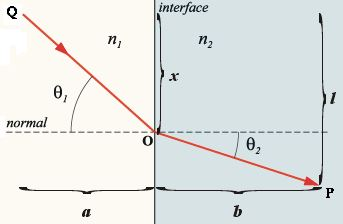
\includegraphics{Fermat.jpg}
\begin{gather*}
    t_{AB} = \frac{\sqrt{a_{x}^{2} + a_{y}^{2}}}{v_{a}} + \frac{\sqrt{b_{x}^{2} + b_{y}^{2}}}{v_{b}} \\
    \frac{dt_{AB}}{db_{x}} = 0 \implies \\
    \frac{dt_{AB}}{db_{x}} = \frac{b_{x}}{v_{a}\sqrt{a_{x}^{2} + a_{y}^{2}}}\frac{da_{x}}{db_{x}} + \frac{b_{x}}{v_{b}\sqrt{b_{x}^{2} + b_{y}^{2}}} \\
    \frac{dt_{AB}}{db_{x}} = \frac{-\sin{\theta_{a}}}{v_{a}} + \frac{\sin{\theta_{b}}}{v_{b}} \\
    \implies n_{a}\sin{\theta_{a}} = n_{b}\sin{\theta_{b}}\text{ -- Snell's Law}
\end{gather*}
\begin{figure}[H]
    \begin{subfigure}{0.3\textwidth}
        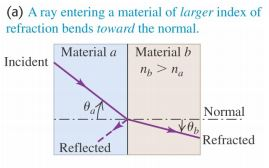
\includegraphics[width=\textwidth]{Refrac1.jpg}
    \end{subfigure}
    \begin{subfigure}{0.3\textwidth}
        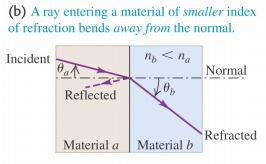
\includegraphics[width=\textwidth]{Refrac2.jpg}
    \end{subfigure}
    \begin{subfigure}{0.3\textwidth}
        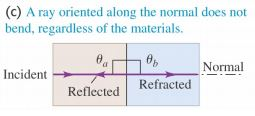
\includegraphics[width=\textwidth]{Refrac3.jpg}
    \end{subfigure}
\end{figure}
Refraction also depends on wavelength:
\begin{gather*}
    v = \lambda f = \frac{c}{n};~f\text{ is unchanged} \\
    \frac{\lambda}{\lambda_{0}} = \frac{v/f}{c/f} = \frac{1}{n}
\end{gather*}

\section{Total Internal Reflection}
Suppose $n_{a} > n_{b}$ (e.g. glass to air) i.e. $v_{a} < v_{b}$, then $\sin{\theta_{b}} = \frac{v_{b}}{v_{a}}\sin{\theta_{a}} > \sin{\theta_{a}}$ \\
When $\sin{\theta_{a}} = \frac{v_{a}}{v_{b}}$, $\theta_{b} = \frac{\pi}{2}$ i.e. all light is reflected past that point \\
For $\theta > \theta_{c} ~\big(\sin{\theta_{c}} = \frac{v_{a}}{v_{b}}\big)$, there is no solution for $\theta_{b}$, so light is totally internally reflected \\
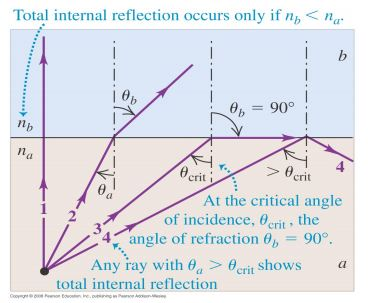
\includegraphics[scale=0.8]{TIR.jpg}

Example: air to glass --
\begin{gather*}
    \sin{\theta_{c}} = \frac{1}{1.52} \approx 0.658 \\
    \theta_{c} \approx 0.229\pi~(\text{Close to }\frac{\pi}{4})
\end{gather*}
Light in glass is totally internally reflected for $\theta > 0.23\pi,~\sin{\theta_{c}} = \frac{n_{b}}{n_{a}}$

\section{Dispersion}
Speed of light in a vacuum is independent of wavelength, but refractive index has variation with wavelength -- this gives dispersion \\
Usually n decreases as $\lambda$ increases \\
This gives prism rainbow effect: \\
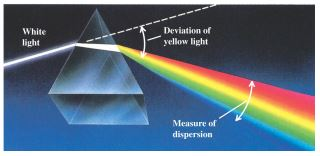
\includegraphics[scale=0.8]{PF.jpg}

\section{Polarisation}
Transverse waves can be polarised, two normals to direction of motion \\
A polarising filter selects a single direction \\
In the electromagnetic spectrum, use \underline{E} to define polarisation:
\begin{equation*}
    \text{y-polarised}
    \begin{cases}
        \underline{E} = \hat{j}E_{max}\cos{(kx - \omega t)} \\
        \underline{B} = \hat{k}B_{max}\cos{(kx - \omega t)}
    \end{cases}
\end{equation*}
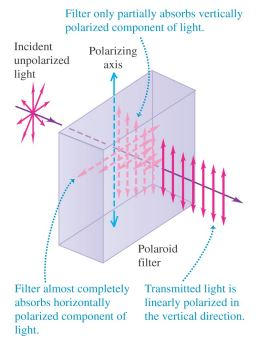
\includegraphics[scale=0.8]{Polarisation.jpg} \\
An ideal polariser would select precisely one polarised component and blocks light perpendicular to this axis \\
For 2 polarisers at an angle: $\underline{E} = E\cos{\phi}\underline{e}_{1} + E\sin{\phi}\underline{e}_{2}$ \\
$\underline{e}_{1}$ is transmitted, $\underline{e}_{2}$ is blocked \\
Transmitted light is most intense when polarisation axes are aligned, blocked when perpendicular \\
Intensity reduced by a factor of $\cos^{2}{\phi}:~I = I_{0}\cos^{2}{\phi}$ -- Malus' Law

\section{Polarisation By Reflection}
For most angles, if \underline{E} is perpendicular to plane of incidence, light is more strongly reflected and partially polarised \\
For \underline{E} in plane of incidence, light more strongly refracted \\
There is a special angle at which no reflection occurs:
\begin{gather*}
    n_{a}\sin{\theta_{a}} = n_{b}\sin{\theta_{b}} \\
    \theta_{a} + \theta_{b} = \frac{\pi}{2} \\
    \tan{\theta_{a}} = \frac{n_{b}}{n_{a}}\text{ -- Brewster Angle}
\end{gather*}
Light polarised completely perpendicular to the plane of incidence is completely reflected

\section{Huygen's principal}
Empirical description rhat captures the essence of wave propagation and works with maths of boundary conditions (reflection/slits/refraction) \\
\emph{"Every point on a primary propagating wavefront serves as a source of spherical secondary wavelets that advance with speed and frequency identical to that of the primary wavefront. The 'next' primary wavefront is the envelope of these seconday wavefronts"}

\section{Ray Tracing}
Ray represents a point on wavefront of light \\
We derive geometric relations for angles at which rays reflect or refract \\
Simple example: plane mirror -- \\
Light rays from P are uniformly reflected and appear to originate from P' \\
Here we trace rays back to P', the rays do not actually pass through P' \\
It is a \emph{virtual image} \\
To find the location of P', note PVB and P'VB are the same (though inverted) triangles $\rightarrow |PV| = |P'V|$ or $|s| = |s'|$
\begin{figure}[H]
    \begin{subfigure}{0.4\textwidth}
        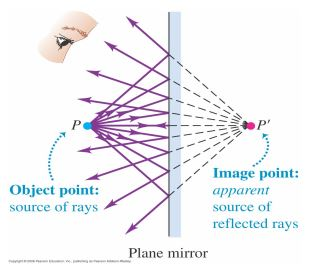
\includegraphics[width=\textwidth]{Mirror1.jpg}
    \end{subfigure}
    \begin{subfigure}{0.4\textwidth}
        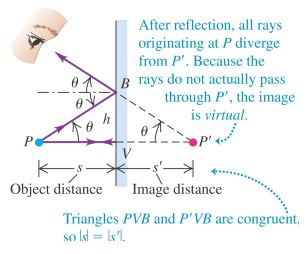
\includegraphics[width=\textwidth]{Mirror2.jpg}
    \end{subfigure}
\end{figure}

\section{Sign Rules}
When $s > 0$, the object is on the incoming side of the surface (i.e. a real object) \\
When $s' > 0$, the object is on the outgoing side of the surface (i.e. virtual object), $s' < 0$ otherwise \\
For a curved surface with a radius of curvature, R: $R > 0$ when centre of curvature is on the outgoing side \\
Lateral magnification: $m > 0$ if image is upright, $m = \frac{y'}{y}$ \\
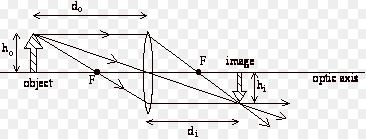
\includegraphics{Lats.jpg}

\section{Spherical Mirror}
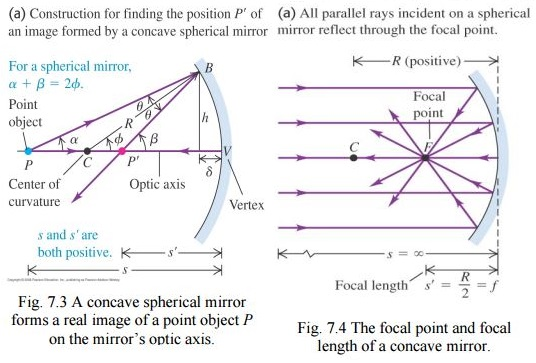
\includegraphics{Mirrors.jpg} \\
C -- centre of curvature; R -- radius of curvature; $\overrightarrow{VC}$ -- principal axis of rotation (mirror is rotationally symmetric around $\overrightarrow{VC}$) \\
Rays parallel to (and close to) VC all reflect through a single point F, the focal point or focus \\
$|VF|$ is the focal length \\
An approximation: rays further out focus closer to mirror (spherical aberration)

\section{Sine Rule and Small Angle Approximation}
\vspace{-18pt}
\begin{gather*}
    \frac{|BC|}{\sin{\alpha}} = \frac{|PC|}{\sin{\theta}} \\
    \frac{R}{\alpha} = \frac{s - R}{\theta} \\
    s = \frac{R}{\alpha}(\alpha + \theta) \\
    \frac{|BC|}{\sin{(\pi - 2\theta - \alpha)}} = \frac{|P'C|}{\sin{\theta}}\\
    \frac{R}{\sin{(2\theta + \alpha)}} = \frac{R}{2\theta + \alpha} = \frac{R - s'}{\theta} \\
    s' = \frac{R(\alpha + \theta)}{\alpha + 2\theta} \\
    \frac{1}{s} = \frac{1}{s'} = \frac{\alpha}{R(\theta + \alpha)} + \frac{\alpha + 2\theta}{R(\theta + \alpha)} = \frac{2}{R} = \frac{1}{f}
\end{gather*}
PQV and P'Q'V: $-\frac{y'}{s'} = \frac{y}{s}$ \\
Similar triangles so $m = \frac{y'}{y} = -\frac{s'}{s}$ \\
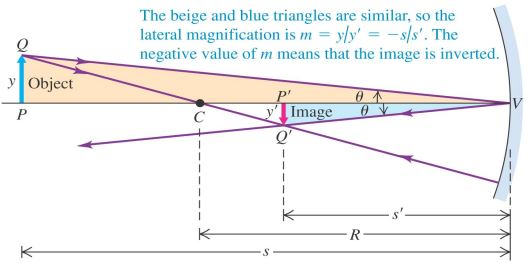
\includegraphics{Reflect1.jpg}

\section{Graphical Method}
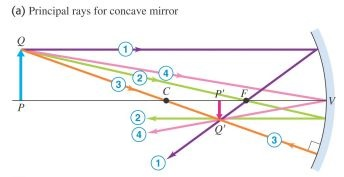
\includegraphics{Reflect2.jpg} \\
Ray parallel to axis reflects throgh focal point ($\frac{R}{2}$); Ray through focal point reflects parallel to axis; Ray through C reflects back on itself; Ray through V reflects symmetrically about axis

\section{Refraction At A Spherical Surface}
Images formed by refraction are our common perception of a lens \\
As before, study a spherical interface: \\
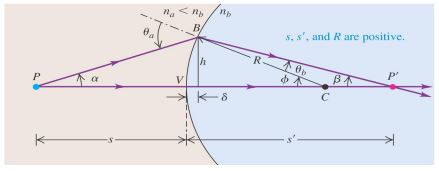
\includegraphics{Refrac4.jpg}
\begin{gather*}
    \beta = \theta_{a} - \theta_{b} - \alpha \\
    \text{From PCB: }\frac{R}{\alpha} = \frac{R}{\sin{\alpha}} = \frac{s + R}{\sin{(\pi - \theta_{a})}} = \frac{s + R}{\theta_{a}} \implies s = (\theta_{a} - \alpha)\frac{R}{\alpha} \\
    \text{From P'CB: }\frac{s' - R}{\sin{\theta_{b}}} = \frac{R}{\sin{\beta}} = \frac{R}{\sin{(\theta_{a} - \theta_{b} - \alpha)}} \implies \frac{R}{\theta_{a} - \theta_{b} - \alpha} \implies s' = \frac{R(\theta_{a} - \alpha)}{\theta_{a} - \theta_{b} - \alpha}
\end{gather*}
\begin{gather*}
    \frac{1}{s'} = \frac{\theta_{a} - (n_{a}\theta_{a}/n_{b}) - \alpha}{(\theta_{a} - \alpha)R} = \frac{1}{n_{b}}\Big[\frac{n_{b}}{R} - \frac{n_{a}\theta_{a}}{R(\theta_{a} - \alpha)}\Big] \\
    \frac{n_{a}}{s} + \frac{n_{b}}{s'} = \frac{n_{b} - n_{a}}{R} \\
    y = s\sin{\theta_{a}} ~\&~ y' = s'\sin{\theta_{b}} \\
    m = -\frac{y'}{y} = \frac{s'}{s}\frac{\sin{\theta_{b}}}{\sin{\theta_{a}}} = \frac{s'}{s}\frac{n_{a}}{n_{b}}
\end{gather*}
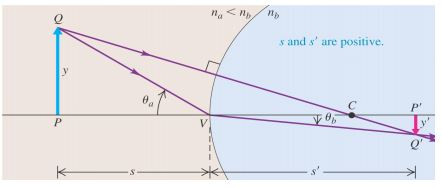
\includegraphics{Refrac5.jpg}

\section{Optical Instruments}
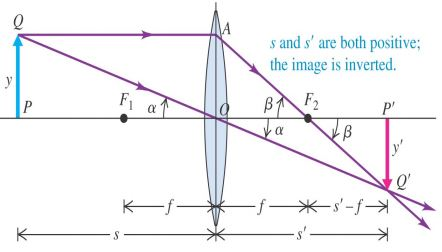
\includegraphics[scale=0.89]{Optic.jpg}

Lens consists of two refracting surfaces \\
Approximately a thin lens by neglecting detail of path inside lens \\
Ray parallel to f is focused at F\textsubscript{2}, ray from F refracted parallel to axis \\
Ray through O is unaffected \\
Real (inverted) image: PQO \& P'Q'O similar, $\frac{y}{s} = -\frac{y'}{s'}$ or $\frac{y'}{y} = \frac{s'}{s}$ \\
OA$F_{2}$ and P'Q'$F_{2}$ similar:
\begin{gather*}
    \frac{y}{f} = -\frac{y'}{s' - f}\text{ or }\frac{y'}{y} = \frac{f - s'}{f} \\
    \text{Together: }-\frac{s'}{s} = \frac{f - s'}{f} \\
    \frac{1}{s} + \frac{1}{s'} = \frac{1}{f}
\end{gather*}
Also applies if lens is diverging \\
Lenses thicker in the middles are converging

\section{The Lensmaker's Equation}
Relation between focal length of lens and radius of curvature and refractive index:
\begin{gather*}
    (1)~~~\frac{n_{a}}{s_{1}} + \frac{n_{b}}{s_{1}'} = \frac{n_{b} - n_{a}}{R_{1}}\\
    (2)~~~\frac{n_{b}}{s_{2}} + \frac{n_{c}}{s_{2}'} = \frac{n_{c} - n_{b}}{R_{2}}
\end{gather*}
Know f is related to Object and Image distances, s \& s'. \\
Object ray first refracts through surface \\
The image (virtual) is object for the second refractive surface: \\ s\textsubscript{1} = s; s\textsubscript{1}' = -s\textsubscript{2} $\therefore$ s\textsubscript{2}' = s' \\
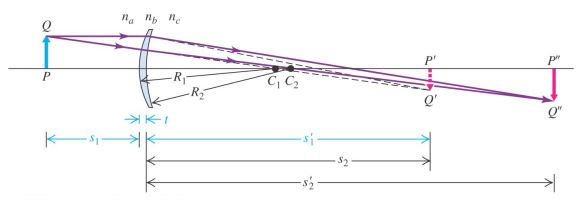
\includegraphics{Lensmaker.jpg}
\begin{gather*}
    (1) + (2) \implies \\
    \frac{n_{a}}{s_{1}} + \frac{n_{c}}{s_{2}^{1}} = \frac{n_{a}}{s} + \frac{n_{a}}{s_{1}} = n_{a}\Big(\frac{1}{s} + \frac{1}{s'}\Big) = LHS \\
    \frac{n_{b} - n_{a}}{R_{1}} + \frac{n_{c} - n_{b}}{R_{2}} = n_{b}\Big(\frac{1}{R_{1}} - \frac{1}{R_{2}}\Big) - n_{a}\Big(\frac{1}{R_{1}} - \frac{1}{R_{2}}\Big) = RHS \\
    \frac{1}{f} = n\Big(\frac{1}{R_{1}} - \frac{1}{R_{2}}\Big) - \Big(\frac{1}{R_{1}} - \frac{1}{R_{2}}\Big) \\
    \underline{\frac{1}{f} = (n - 1)\Big(\frac{1}{R_{1}} - \frac{1}{R_{2}}\Big)}
\end{gather*}
Examples of lenses: \underline{Camera} -- \\
Camera consists of a lens, shutter, receptor, \& aperture control \\
Intensity of light on film is proportional to area viewed by camera \\
Aperture controls area $\propto D^{2}$ \\
$I \propto \frac{D^{2}}{f^{2}}$ -- f number $= \frac{f}{D}$

\section{Interference}
Interference occurs when waves overlap, as with mechanical waves, we use principal of superposition \\
If two or more wabes overlap, we add wave functions
\begin{gather*}
    Q(\underline{x},\,t) = Q_{1}(\underline{x},\,t) + Q_{2}(\underline{x},\,t)
\end{gather*}
Apply to light: electromagnetic waves
\begin{gather*}
    \text{Rep: }\underline{E} = \underline{E}_{0}\cos{(\underline{k}\cdot\underline{x} - \omega t)} \\
    \underline{E}_{0}\text{ -- polarisation and amplitude; }A = |E_{0}| \\
    \underline{k}\text{ -- wave-vector direction of travel} \\
    \underline{k}\cdot\underline{E}_{0} = 0
\end{gather*}
Consider monochromatic coherent light:
\begin{gather*}
    \underline{E}_{i}\cos{(\underline{k}_{i}\cdot\underline{x} - \omega t)}~~\{i \in \mathbb{N}\} \\
    k\text{ -- possibly different} \\
    \omega\text{ -- the same }\forall ~i
\end{gather*}
Consider two sources of monochromatic light with the same amplitude: \\
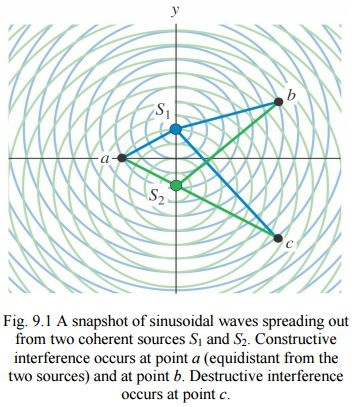
\includegraphics{Construc.jpg}
\begin{gather*}
    \text{Constructive: }|\overrightarrow{S_{1}P}| = |\overrightarrow{S_{2}P}| - n\lambda \\
    r_{2} - r_{1} = n\lambda, ~\{n \in \mathbb{Z}\} \\
    \text{Destructive: }r_{2} - r_{1} = \Big(n + \frac{1}{2}\Big)\lambda
\end{gather*}
Lines of constructive interference are antinodal lines \\
Lines of destructive interference are nodal lines

\section{Young's Slits}
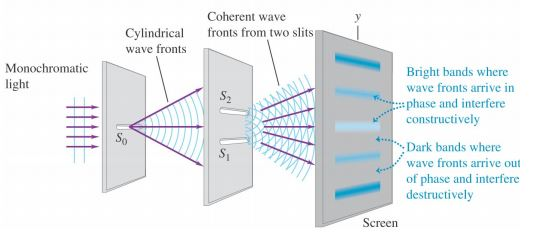
\includegraphics{Young1.jpg} \\
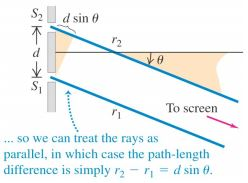
\includegraphics{Young2.jpg} \\
$R << d \therefore \theta$ is small \\
Extra distance for first ray gives phase difference $= d\sin{\theta} \approx d\theta$ \\
For constructive interference: $n\lambda = d\theta~(d\sin{\theta})$ \\
Distance between fringes for the n\textsuperscript{th} fringe:
\begin{gather*}
    y_{n} = R\tan{\theta_{n}} \approx R\theta_{n} \\
    ~~~\, = R\frac{n\lambda}{d}
    n\lambda = \frac{y_{n}d}{R}
\end{gather*}
Intensity is proportional to $A^{2}$:\\
For a single electromagnetic wave --
\begin{equation*}
    I = \frac{1}{2}cE^{2}\epsilon_{0}\text{ -- E is amplitude}
\end{equation*}
How to add out-of-phase \& differing amplitude? (still monochromatic)
\begin{equation*}
    E_{1}\cos{(\omega t)} + E_{2}\cos{(\omega t + \phi)}
\end{equation*}
There are two different methods that can be used: \\
(1) -- Algebra
\begin{gather*}
    E\cos{(\omega t + \alpha)} = E_{1}\cos{(\omega t)} + E_{2}\cos{(\omega t + \phi)} \\
    = E_{1}\cos{(\omega t + \alpha - \alpha)} + E_{2}\cos{(\omega t + \alpha + \phi - \alpha)} \\
    = E_{1}\cos{(\omega t + \alpha)}\cos{\alpha} + E_{1}\sin{(\omega t + \alpha)}\sin{\alpha} + E_{2}\cos{(\omega t + \alpha)}\cos{(\phi - \alpha)} - E_{2}\sin{(\omega t + \alpha)}\sin{(\phi - \alpha)} \\
    = [E_{1}\cos{\alpha} + E_{2}\cos{(\phi - \alpha)}]\cos{(\omega t + \alpha)} + [E_{1}\sin{\alpha} - E_{2}\sin{(\phi - \alpha)}]\sin{(\omega t + \alpha)}
\end{gather*}
Choose $\alpha$ to set 2\textsuperscript{nd} term to zero:
\begin{gather*}
    E_{1}\sin{\alpha} = E_{2}\sin{(\phi - \alpha)} = E_{2}\sin{(\sin{\phi}\cos{\alpha} - \cos{\phi}\sin{\alpha})} \\
    \implies \tan{\alpha} = \frac{E_{2}\sin{\phi}}{E_{1} + E_{2}\cos{\phi}}\\
    \text{Check: } E_{1} = E_{2}\\
    \implies \tan{\alpha} = \frac{\sin{\phi}}{1 + \cos{\phi}} = \frac{2\sin{\phi/2}\cos{\phi/2}}{2\cos^{2}{\phi/2}} = \tan{\frac{\phi}{2}} \\
    \implies \alpha = \frac{\phi}{2}
\end{gather*}
(2) -- Phasors \\
Represent the wave by a rotating vector \\
To add waves, add vectors \\
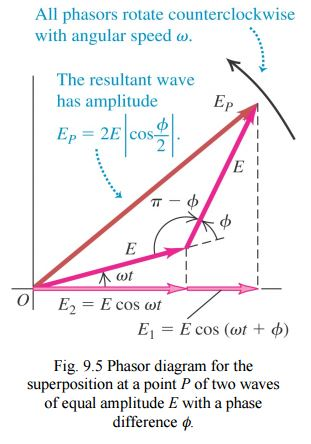
\includegraphics{Phasors.jpg}\\
From vector addition:
\begin{gather*}
    E_{1}\cos{(\omega t)} + E_{2}\cos{(\omega t + \phi)}
\end{gather*}
Find $\alpha$ at $t = 0$:
\begin{gather*}
    E_{y} = E_{2}\sin{\phi} = E\sin{\alpha} \\
    E_{x} = E_{1} + E_{2}\cos{\phi} \\
    E^{2} = (E_{1} + E_{2}\cos{\phi})^{2} + E_{2}^{2}\sin^{2}{\phi} \\
    ~~~\, = E_{1}^{2} + E_{2}^{2} + 2E_{1}E_{2}\cos{\phi} \\
    E\sin{\alpha} = E_{2}\sin{\phi} \\
    \implies \tan{\alpha} = \frac{E_{2}\sin{\phi}}{E\cos{\alpha}} = \frac{E_{2}\sin{\phi}}{E_{1} + E_{2}\cos{\phi}}
\end{gather*}

\section{Intensity In Interference}
Intensity of a electromagnetic wave:
\begin{equation*}
    I = \frac{1}{2}\epsilon_{0}cE^{2} = \frac{1}{2}\sqrt{\frac{\epsilon_{0}}{\mu_{0}}}E^{2}
\end{equation*}
For 2 waves of the same amplitude, $E_{tot} = 2E\cos{\Big(\frac{\phi}{2}\Big)}$:
\begin{equation*}
    I = \Big(2E\cos{\Big(\frac{\phi}{2}\Big)}\Big)^{2} \frac{\epsilon_{0}c}{2} = 4I_{0}\cos^{2}{\Big(\frac{\phi}{2}\Big)}
\end{equation*}
Max intensity for $\phi = 0$\\
Average over all phase angles:
\begin{gather*}
    \langle I\rangle = \frac{I_{0}}{2\pi}\int_{0}^{2\pi}\cos^{2}{\Big(\frac{\phi}{2}\Big)}\, d\phi \\
    \implies \frac{4I_{0}}{2\pi}\int_{0}^{2\pi}\frac{1 + \cos{\phi}}{2}\, d\phi = 2I_{0}
\end{gather*}
Intensity in interference is redistributed: \\
Central peak has intensity $4I_{0}$ here \\
Can relate phase to path length:
\begin{equation*}
    \phi = \frac{2\pi}{\lambda}(r_{2} - r_{1})
\end{equation*}
For Young's Slits:
\begin{gather*}
    r_{2} - r_{1} = d\sin{\theta} = \frac{dy}{R} \\
    \phi = kd\sin{\theta} = \frac{2\pi d}{\lambda}\sin{\theta} \\
    I = I_{0}\cos^{2}{\Big(\frac{1}{2}kd\sin{\theta}\Big)} \\
    I = 4I_{0}\cos^{2}{\Big(\frac{kdy}{2R}\Big)}
\end{gather*}

\section{Interference In Thin Films}
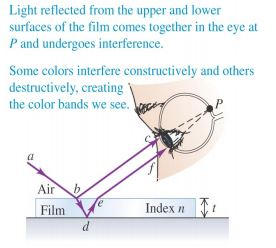
\includegraphics{Film.jpg} \\
Light reflected from both interfaces has a phase difference giving interference \\
Inteference depends on $\lambda$, so see different colours at different angles

\section{Phase \& Reflection}
When light hits a surface, typically some is reflected and some is refracted \\
The amount reflected depends on the angle of incidence, refractive indices, and polarisations \\
For nearly normal incidence, $E_{r} = \frac{n_{a} - n_{b}}{n_{a} + n_{b}}E_{i}$ \\
Although E is typically positive, keeping this as $n_{a} - n_{b}$ tells us about phase shift \\
Analogous to reflected and transmitted mechanical waves
\begin{gather*}
    [I\cos{(k_{1}x - \omega t)} + R\cos{(k_{1}x - \omega t)}] + T\cos{(k_{2}x - \omega t)} \\
    v_{1/2} = \frac{\omega}{k_{1/2}} \\
    \text{At }x = 0:~y = I\cos{(\omega t)} + R\cos{(\omega t)} = T\cos{(\omega t)} \\
    I + R = T \\
    y' = -Ik_{1}\sin{(-\omega t)} - Rk_{1}\sin{\omega t} = -Tk_{2}\sin{(-\omega t)} \\
    k_{2}T = k_{1}(I - R) \\
    T = I + R = \frac{k_{1}}{k_{2}}(I - R) \\
    R = \frac{k_{1} - k_{2}}{k_{1} + k_{2}}I
\end{gather*}
$n_{a} < n_{b}$ -- phase shift of $\pi$ in reflected light \\
If neither/both reflected waves have a phase shift, then the path difference gives the phase shift. \\
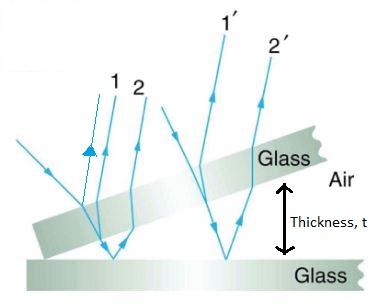
\includegraphics[scale=0.8]{Thickness.jpg} \\
Otherwise:
\begin{equation*}
    \phi = \frac{2\pi}{\lambda}(r_{2} - r_{1}) + \pi
\end{equation*}
\begin{gather*}
    2t = n\lambda \text{ -- constructive, no phase shift} \\
    2t = \Big(n + \frac{1}{2}\Big)\text{ -- destructive, phase shift}
\end{gather*}

\section{Michelson Interferometer}
Exploits interference effects by splitting monochromatic light, sending on different paths, then recombing and looking for phases shifts \\
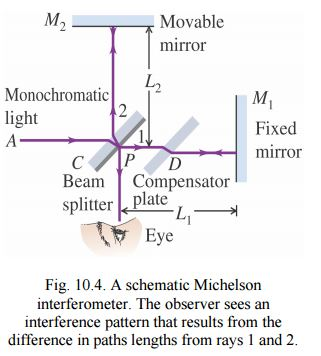
\includegraphics[scale=0.8]{Michelson.jpg} \\
Compensator plate ensures both light paths travel through same amount of glass \\
In essence, same set-up as LIGO

\section{Diffraction}
\emph{Wave nature of light means that boundaries do not cast precisely sharp shadows. Light "bends" around corners, and a close look reveals patterns of interference} \\
Full problem includes solving wave equation subject to boundary conditions (meaning wave from slits) \\
Near-region diffraction is Fresnal \\
Far-field is Fraunhofer

\section{Fraunhofer Diffraction}
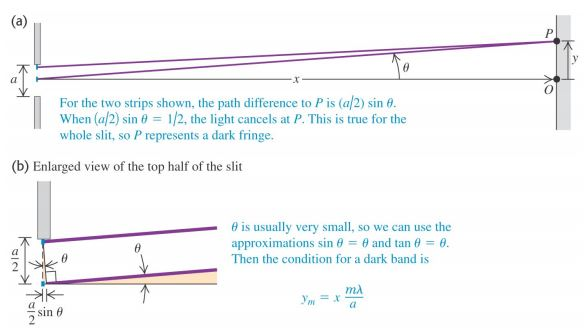
\includegraphics{Fraunhofer.jpg} \\
Path difference: $r_{2} - r_{1}$
\begin{equation*}
    r_{2} - r_{1} \approx \frac{a}{2}\sin{\theta}
\end{equation*}
Destructive interference if $\frac{a}{2}\sin{\theta} = n\frac{\lambda}{2}$ \\
Expect dark fringes around a central bright band \\
Break slit into 4: \\
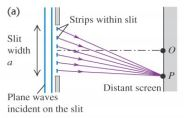
\includegraphics[scale=1.6]{Diffrac1.jpg} \\
Path difference of $\frac{a}{4}\sin{\theta}$ between successive rays \\
Destructive at $\frac{a}{4}\sin{\theta} = \frac{\lambda}{2}$ \\
Expect dark fringes at $a\sin{\theta} = n\lambda$ \\
To find actual result, combine wavefronts from all points between $-\frac{a}{2}$ and $\frac{a}{2}$
\begin{equation*}
    r_{2} - r_{1} = y\sin{\theta}
\end{equation*}
Add up combination from $y \in {[{-\frac{a}{2}},\frac{a}{2}]}$ \\
Integrate phase difference across slits:
\begin{equation*}
    \frac{1}{a} \int_{-a/2}^{a/2} \cos{(ky\sin{\theta})}\,dy
\end{equation*}
($ky\sin{\theta}$ is the phase at y)
\begin{gather*}
    = \frac{1}{a} \int_{-a/2}^{a/2} \cos{(ky\sin{\theta})}\,dy \\
    = \frac{1}{a} \Big[\frac{\sin{(ky\sin{\theta})}}{k\sin{\theta}}\Big]^{a/2}_{-a/2} \\
    = \frac{1}{ak\sin{\theta}} \Big[\sin{\Big(\frac{ka}{2}\sin{\theta}\Big)} - \sin{\Big(-\frac{ka}{2}\sin{\theta}\Big)}\Big] \\
    = \frac{2}{ak\sin{\theta}}\sin{\Big(\frac{ka}{2}\sin{\theta}\Big)} \\
    = \frac{\sin{\big(\tfrac{ka}{2}\sin{\theta}\big)}}{\tfrac{ka}{2}\sin{\theta}}\\
    = \frac{\sin{x}}{x},~~x = \frac{ka}{2}\sin{\theta}
\end{gather*}
Diffraction depends on:
\begin{itemize}
    \item[] $k = \frac{2\pi}{\lambda}$, i.e. wavelenghts
    \item[] a, the width of the slit
    \item[] $\sin{\theta}$, where we are on the screen
\end{itemize}
This gives our amplitude, so intensity patter is:
\begin{equation*}
    I = I_{0}\Bigg(\frac{\sin{\big(\tfrac{ka}{2}\sin{\theta}\big)}}{\tfrac{ka}{2}\sin{\theta}}\Bigg)^{2}
\end{equation*}
At $\theta = 0$ (centre of the screen), $\frac{\sin{x}}{x} \rightarrow 1$ \\
$\implies$ Intensity is maximum, $I =I_{0}$ \\
1\textsuperscript{st} Dark Fringe at (multiply RHS by n for other fringes):
\begin{gather*}
    \frac{ka}{2}\sin{\theta} = \pi \\
    \frac{a\pi}{\lambda}\sin{\theta} = \pi \\
    a\sin{\theta} = \lambda
\end{gather*}

\section{Phasor Derivation}
Split the slit into N source-lets and add the wave vectors for each
\begin{itemize}
    \item[] Amplitude for each source -- $\frac{A}{N}$
    \item[] Phase -- $\frac{2\pi}{\lambda}\frac{a}{N}\sin{\theta} = \frac{ka}{N}\sin{\theta}$
\end{itemize}
\begin{figure}[H]
    \begin{subfigure}{0.4\textwidth}
        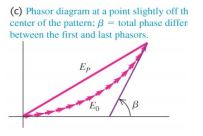
\includegraphics[width=\textwidth]{Phas1.jpg}
    \end{subfigure}
    \begin{subfigure}{0.4\textwidth}
        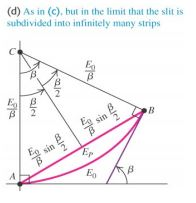
\includegraphics[width=\textwidth]{Phas2.jpg}
    \end{subfigure}
\end{figure}
As $N \rightarrow \infty$, the phasors succesively approximate an arc \\
Total phase is always $\beta = ka\sin{\theta}$ \\
Total amplitude, $A_{T} = \frac{2A}{\beta}\sin{\Big(\frac{\beta}{2}\Big)}$

\section{Diffraction and Interference}
Young's slits with finite width: \\
For 2 slits we found that --
\begin{gather*}
    E = 2E_{0}\cos{\Big(\frac{kd}{2}\sin{\theta}\Big)} \\
    I = 2I_{0}\cos^{2}{\Big(\frac{kd}{2}\sin{\theta}\Big)}
\end{gather*}
and for diffraction:
\begin{equation*}
    E = E_{0}\frac{\sin{\big(\tfrac{ka}{2}\sin{\theta}\big)}}{\tfrac{ka}{2}\sin{\theta}}
\end{equation*}
principal of superpositions means we superpose these effects --
\begin{gather*}
    E = E_{0}\frac{\sin{\big(\tfrac{ka}{2}\sin{\theta}\big)}}{\tfrac{ka}{2}\sin{\theta}}\Big[2\cos{\Big(\frac{kd}{2}\sin{\theta}\Big)}\Big],~d = 4a \\
    E = E_{0}\frac{\sin{\big(\tfrac{ka}{2}\sin{\theta}\big)}}{\tfrac{ka}{2}\sin{\theta}}\Big[2\cos{\Big(2ka\sin{\theta}\Big)}\Big]
\end{gather*}
The 4\textsuperscript{th} maximum of interference is deleted by a minimum of the diffraction envelope

\section{Circular Apertures and Resolving Power}
Any shape aperture forms a diffraction pattern \\
A circular aperture is common and forms an "Airy Disk" \\
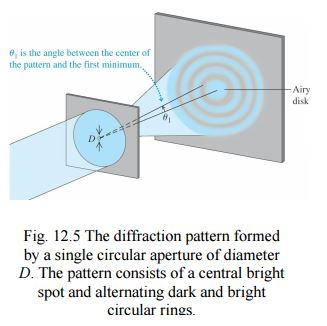
\includegraphics{Airy.jpg} \\
For cylindrical or spherical wavefronts, we replace sin/cos by Bessel functions:
\begin{equation*}
    I = I_{0}\Bigg(2\frac{J_{1}\big(\tfrac{kD}{2}\sin{\theta}\big)}{\tfrac{kD}{2}\sin{\theta}}\Bigg)^{2}
\end{equation*}
$J_{1}$ is a Bessel function; D is the diameter of the aperture
\begin{gather*}
    \text{First zero at }\frac{kD}{2}\sin{\theta} \approx 1.22\pi \\
    \text{Or }\theta \approx 1.22\frac{\lambda}{D}
\end{gather*}
Sets limits on optical resolution \\
Need big D or smaller $\lambda$

\section{Diffraction with Multiple Slits}
What happens with many slits? \\
Look at $N = 4$ \\
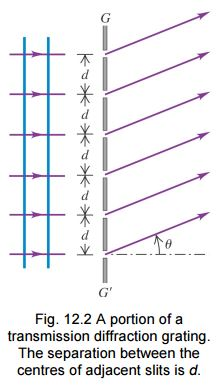
\includegraphics[scale=0.8]{Grating.jpg} \\
Path difference is $d\sin{\theta}$ \\
If $d\sin{\theta} = n\lambda$, set constructive interference from all 4 sources: \\
Let $\phi = kd\sin{\theta}$ -- phase shift for adjacent sources \\
$r_{0}$ -- distance of source to screen; $E_{0}$ -- amplitude of one source \\
Overall amplitude:
\begin{gather*}
    E_{tot} = E_{0}[\cos{(kr_{0})} + \cos{(kr_{0} + \phi)} + \cos{(kr_{0} + 2\phi)} + \cos{(kr_{0} + 3\phi)}] \\
    E_{tot} = E_{0}\bigg[2\cos{\big(kr_{0} + \tfrac{\phi}{2}\big)}\cos{\big(\tfrac{\phi}{2}\big)} + 2\cos{\big(kr_{0} + \tfrac{5\phi}{2}\big)}\cos{\big(\tfrac{\phi}{2}\big)}\bigg] \\
    E_{tot} = 2E_{0}\cos{\big(\tfrac{\phi}{2}\big)}\bigg[2cos{\big(kr_{0} + \tfrac{3\phi}{2}\big)}\cos{(\phi)}\bigg] \\
    E_{tot} = 4E_{0}\cos{\big(\tfrac{\phi}{2}\big)}\cos{(\phi)}\cos{\big(kr_{0} + \tfrac{3\phi}{2}\big)}
\end{gather*}
The 4 slits combine to give total amplitude:
\begin{gather*}
    E_{tot} = 4E_{0}\cos{\big(\tfrac{\phi}{2}\big)}\cos{(\phi)} \\
    \phi = 2\pi n \\
    E_{tot} = 4E_{0}
\end{gather*}
All 4 sources constructively interfere \\
But have $E_{tot} = 0$ for $\phi = \frac{n\pi}{2}$ \\
Intensity $\propto E_{tot}^{2}$ \\
Evenly spcaed dark fringes at:
\begin{equation*}
    kd\sin{\theta} = \frac{2\pi}{n},~n \in \mathbb{N}
\end{equation*}
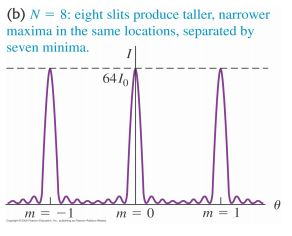
\includegraphics{Intense.jpg} \\
Added amplitudes out of phases -- can use phasors \\
Easy to find dark fringes for $N = 4$ by adding vectors of phase differences \\
Deduce local maximums from this \\
For N slits, get principal maxima of intensity:
\begin{equation*}
    I = N^{2}I_{0}\text{ -- Very Sharp Peak}
\end{equation*}
For dark fringe, $\phi = \frac{2\pi}{N},~\frac{4\pi}{N} ...\rightarrow \frac{2(N - 1)\pi}{N}$ \\
So we have (N - 1) dark fringes between principal maxima \\
Local maxima are much lower \\
Also can get a diffraction envelope superposed if slit width is 'significant'

\section{Diffraction Grating and X-Ray Diffraction}
An array of a large number of parallel slits with same spacing, d, and width, a, is a diffraction grating \\
Principal maxima occur at $d\sin{\theta} = n\lambda$ produce sharp maxima \\
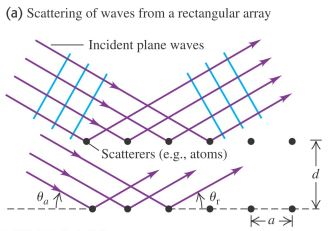
\includegraphics{Grat1.jpg} \\
Consider X-rays incident on a 2D array of atoms \\
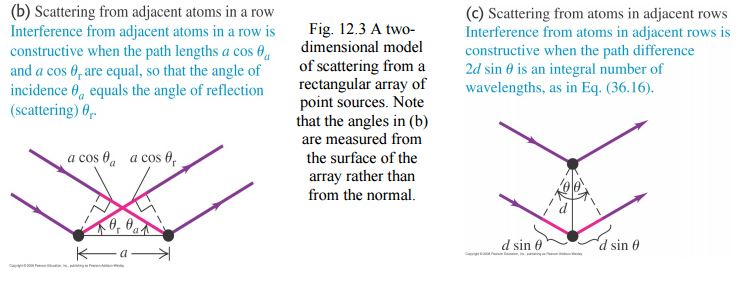
\includegraphics[width=\textwidth]{Scatter.jpg} \\
Total path length the same for $\theta_{r} = \theta_{a}$ \\
Looked at scatter for adjacent rows also \\
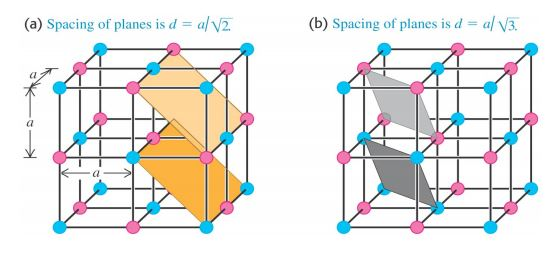
\includegraphics{Crystals.jpg}
\end{document}
